\chapter{Frobenius' Conjecture and Markov Numbers}
In number theory, more precisely, in the theory of Diophantine equations, one that is of particular interest is \emph{Markov's equation};
\begin{equation}\label{Markov}
    x^2 + y^2 + z^2 = 3xyz.
\end{equation}
A triple $(a,b,c), \ a \leq b \leq c$, that is a solution to (3.1) is called a \emph{Markov triple}, and $a,b,$ and $c$ are called \emph{Markov numbers}. A few of these are $(1,1,1),(1,1,2), (1,2,5), (1,5,13)$, $(1, 89, 233), (5, 29, 433)$. It is known that every other Fibonacci number is a Markov number, and so is every Pell number. The essence of Frobenius' conjecture is that of uniqueness of solutions;
\begin{conjecture}[Frobenius' Uniqueness Conjecture]
    Let $(a_1,a_2,\tau)$ and $(b_1,b_2,\tau)$ be Markov triples, then $a_1 = b_1$ and $a_2=b_2$. 
\end{conjecture}

\section{Markov generating function}
We begin by considering the torus $\mathcal{T}^2$ as the quotient space
\begin{equation*}
    \mathcal{T}^2 \cong \mathcal{I}\times \mathcal{I}/\sim_{ns} \sim_{we},
\end{equation*}
where $\mathcal{I} = [0,1] \subseteq \mathbb{R}$, and $\sim_{ns}, \sim_{we}$ are the equivalence relations identifying \emph{north} with \emph{south} and \emph{west} with \emph{east}. Next, we triangulate it; which is much easier to do when viewing it via the quotient (as it is simply a diagonal) than as a 3-dimensional manifold; and then we remove a single point, more precisely the point $(0,0) \sim (0,1)\sim (1,0) \sim (1,1)$. In the figure below, we have the following image.
\begin{figure}[H]
    \centering
    \includegraphics[width = 5 cm]{figures/Torus.tex}
    \label{Torus}
    \caption{Triangulated torus $\mathcal{T}^2$.}
\end{figure}
After we label each side (of which there are 3) we fix a \emph{clockwise orientation}; i.e. as we approach where two diagonals meet, the orientation is as follows;
\begin{figure}[H]
    \centering


    \tikzset{every picture/.style={line width=0.75pt}} %set default line width to 0.75pt        

    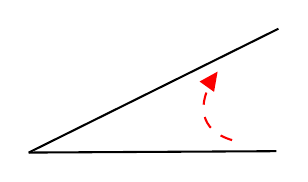
\begin{tikzpicture}[x=0.75pt,y=0.75pt,yscale=-1,xscale=1]
    %uncomment if require: \path (0,487); %set diagram left start at 0, and has height of 487
    
    %Straight Lines [id:da4370862379579007] 
    \draw    (120.17,250.5) -- (240.5,190.83) ;
    %Straight Lines [id:da8355747741827015] 
    \draw    (120.17,250.5) -- (239.5,249.83) ;
    %Curve Lines [id:da10366436706962945] 
    \draw [color={rgb, 255:red, 251; green, 0; blue, 0 }  ,draw opacity=1 ] [dash pattern={on 4.5pt off 4.5pt}]  (218.17,244.5) .. controls (202.1,239.78) and (201.22,227.01) .. (209.61,213.81) ;
    \draw [shift={(211.17,211.5)}, rotate = 125.54] [fill={rgb, 255:red, 251; green, 0; blue, 0 }  ,fill opacity=1 ][line width=0.08]  [draw opacity=0] (8.93,-4.29) -- (0,0) -- (8.93,4.29) -- cycle    ;
    
    
    
    
    \end{tikzpicture}

    
    
\end{figure}
If we then apply it to our construction, we obtain the following;

\begin{figure}[!htb]
\centering
\minipage[c]{0.375\textwidth}
\footnotesize
\includegraphics[width = 6 cm]{figures/TriangTorusMP.tex}
\endminipage\hfill
\minipage[c]{0.25\textwidth}
\centering
\footnotesize
\tikzset{every picture/.style={line width=0.75pt}}
\begin{tikzpicture}[x=0.75pt,y=0.75pt,yscale=-1,xscale=1]
\draw    (105,190) .. controls (187.17,81.5) and (98.17,245.5) .. (230.17,182.5) ;
\draw [shift={(230.17,182.5)}, rotate = 154.49] [color={rgb, 255:red, 0; green, 0; blue, 0 }  ][line width=0.75]    (21.86,-6.58) .. controls (13.9,-2.79) and (6.61,-0.6) .. (0,0) .. controls (6.61,0.6) and (13.9,2.79) .. (21.86,6.58)   ;
\end{tikzpicture}
\endminipage\hfill
\minipage[c]{0.375\textwidth}%
\footnotesize
\includegraphics[width = 6 cm]{figures/TriangTorusMPOrient.tex}
\endminipage
\end{figure}
Observe that now we have precisely 2 arrows $1 \rightarrow 3$, 2 arrows $3 \rightarrow 2$ and 2 arrows $2 \rightarrow 1$; which we can then us to construct the following quiver $\mathcal{Q}$;
\begin{figure}[H]
    \centering
   \begin{tikzcd}
	&& 2 \\
	\\
	\\
	1 &&&& 3
	\arrow[shift left=1, from=1-3, to=4-1]
	\arrow[shift left=1, from=4-1, to=4-5]
	\arrow[shift left=1, from=4-5, to=1-3]
	\arrow[shift right=1, from=1-3, to=4-1]
	\arrow[shift right=1, from=4-1, to=4-5]
	\arrow[shift right=1, from=4-5, to=1-3]
\end{tikzcd}
\end{figure}
This is also known as the \emph{Markov quiver}. Let $\mathbf{x} = (x_1,x_2,x_3)$, and $\mathbf{y} = (1,1,1)$; then define the seed $(\mathbf{x},\mathbf{y},\mathcal{Q})$ and consider the mutation $\mu_1$.\footnote{Vertex 1 is obviously arbitrary, and we could have taken $\mu_2$ or $\mu_3$ without yielding \emph{meaningfully} different results.} Recall that since $\mathbf{y}$ is a vector of 1's, we can leave it out throughout our calculations. Consequently, we obtain that $x_1^{'} = (x_2^2 + x_3^2)/x_1$; and through (\ref{Markov}), $x_1^{'} = 3x_2x_3 - x_1$; i.e. $\mu_1$ acts on a triple $(x,y,z)$ by 
\begin{equation}
    (x,y,z) \xrightarrow{\mu_1} (3yz-x,y,z).
\end{equation}
Via a method called \emph{Vieta jumping}, or equivalently \emph{root flipping}, one can show that if $(x,y,z)$ is a Markov triple then $\mu_1(x,y,z) = (3yz-x,y,z)$ is also a Markov triple. Infact, begin with $(x,y,z) = (1,1,1)$, then
\begin{align*}
    \mu_1(1,1,1) &= (2,1,1) \sim (1,1,2), \\
    \mu_1(1,1,2) &= (5,1,2) \sim (1,2,5), \\
    \mu_1(1,2,5) &= (29,2,5) \sim (2,5,29), \\
    \mu_1(2,5,29) &= (433,5,29) \sim (5,29,433), \\
    & \ \vdots
\end{align*}
If we apply it to all Markov triples, we can construct a branch of the \emph{Markov Number Tree};
\begin{figure}[H]
    \centering
    \includegraphics[width = 12 cm]{figures/MarkovNumberTree.tex}
\end{figure}
 The same process can be done to yield two the other mutations $\mu_2,\mu_3$. Similarly, for all three we have that if we start with a Markov triple $(x,y,z)$, then $\mu_i(x,y,z)$ is also a Markov triple. However, $\mu_i(x,y,z)$ need not be equal to $\mu_j(x,y,z)$, for $i \ne j$. For example, if we take $\mu_2$ (the reader might like to prove that $(x,y,z) \xrightarrow{\mu_2} (x,3xz-y,z)$) we can see that;
\begin{equation*}
    \mu_2(1,2,5) = (1,13,5) \sim (1,5,13) \ne (2,5,19) = \mu_1(1,2,5).
\end{equation*}
Meaning that we can go from triple to triple by a sequence of these mutations. Additionally, the resulting quiver, after any sequence of these mutations, becomes;
\begin{figure}[H]
    \centering
    \[\begin{tikzcd}
	&& 2\\
	\\
	\\
	1 &&&& 3
	\arrow[shift left=1, from=4-1, to=1-3]
	\arrow[shift right=1, from=4-1, to=1-3]
	\arrow[shift left=1, from=1-3, to=4-5]
	\arrow[shift right=1, from=1-3, to=4-5]
	\arrow[shift left=1, from=4-5, to=4-1]
	\arrow[shift right=1, from=4-5, to=4-1]
\end{tikzcd}\]
\end{figure}
which is clearly just the initial Markov quiver simply with all arrows inverted. This yields the following corollary;
\begin{corollary}
The Markov quiver has a single equivalence class with respect to cluster mutations.
\end{corollary}

\section{Markov Numbers}
As seen in the previous section, Markov triples are related to the clusters of the cluster algebra corresponding to the once-punctured torus. As the cluster variables are computed by snake graphs, we can view Markov numbers in terms of snake graphs. 